\chapter{Lec 08 - Logical Agents}
\section{Logical Agents}
Logical agents simulate the process of \textbf{reasoning} operating on internal \textbf{representations} of knowledge. The problem-solving agents seen so far know things, but only in a very limited,
inflexible sense. The knowledge of what the actions do is hidden inside the domain-specific code of the transition model, which defines the result of a move. We will see that \textbf{logic} provides a possible formalism to support knowledge-based agents.

\section{Knowledge based agents}
The central component of a knowledge-based agent is its \textbf{knowledge base}, or KB. A knowledge base is a set of \textbf{sentences} in a formal language. Each sentence is expressed in a language called a \textbf{knowledge representation language} and represents some assertion about the world.\newline\newline
There must be a way to add new sentences to the knowledge base and a way to query what is known. The standard names for these operations are TELL and ASK, respectively. Both operations may involve inference, that is, deriving new sentences from old.\newline\newline
Agents can be viewed at the \textbf{knowledge level}, that is, what they know, regardless of how implemented, or can be viewed  at the implementation level, data structures in KB and algorithms that manipulate them.
\begin{center}
    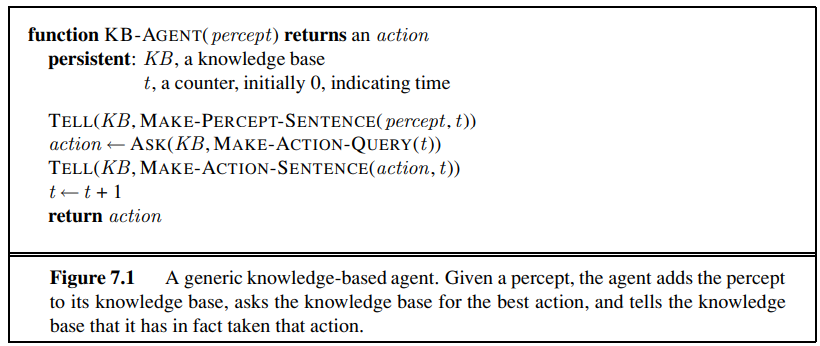
\includegraphics[]{images/KB-agents.png}
\end{center}
The figure above shows the outline of a knowledge-based agent program. Like all our agents, it takes a percept as input and returns an action. The agent maintains a knowledge base, KB, which may initially contain some \textbf{background knowledge}.\newline\newline
Each time the agent program is called, it does three things. First, it TELLs the knowledge base what it perceives. Second, it ASKs the knowledge base what action it should perform. In the process of answering this query, extensive reasoning may be done about the current state of the world, about the outcomes of possible action sequences, and so on.
Third, the agent program TELLs the knowledge base which action was chosen, and the agent executes the action. In order to do so, the agent must be able to:
\begin{itemize}
    \item Represent states, actions, etc.
    \item Incorporate new percepts
    \item Update internal representations of the world
    \item Deduce hidden properties of the world
    \item Deduce appropriate actions
\end{itemize}

\section{The Wumpus world}
In this section we describe an environment in which knowledge-based agents can show their worth. The \textbf{wumpus world} is a cave consisting of rooms connected by passageways. Lurking somewhere in the cave is the terrible wumpus, a beast that eats anyone who enters its room. The wumpus can be shot by an agent, but the agent has only one arrow. Some rooms contain bottomless pits that will trap anyone who wanders into these rooms (except for the wumpus, which is too big to fall in). The only mitigating feature of this bleak environment is the possibility of finding a heap of gold.
\begin{center}
    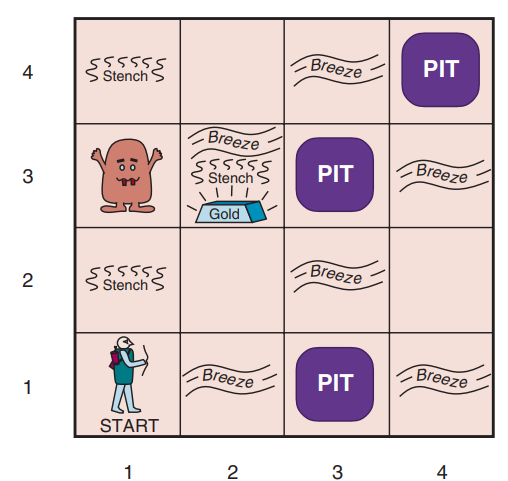
\includegraphics[]{images/wumpus.png}
\end{center}
The precise definition of the task environment is given by the PEAS description:
\begin{itemize}
    \item \textbf{Performance measure}: +1000 for climbing out of the cave with the gold, -1000 for falling into a pit or being eaten by the wumpus, -1 for each action taken and -10 for using up the arrow. The game ends either when the agent dies or when the agent climbs out of the cave.

    \item \textbf{Environment:} A $4 \times 4$ grid of rooms. The agent always starts in the square labeled $[1,1]$, facing to the right. The locations of the gold and the wumpus are chosen randomly, with a uniform distribution, from the squares other than the start square. In addition, each square other than the start can be a pit, with probability 0.2.

    \item \textbf{Actuators:} The agent can move \textit{Forward}, \textit{TurnLeft} by $90^{\circ}$, or \textit{TurnRight} by $90^{\circ}$. The agent dies a miserable death if it enters a square containing a pit or a live wumpus. The action \textit{Grab} can be used to pick up the gold if it is in the same square as the agent. The action \textit{Shoot} can be used to fire an arrow in a straight line in the direction the agent is facing (only one available). Finally, the action \textit{Climb} can be used to climb out of the cave, but only from square $[1,1]$.

    \item \textbf{Sensors:} The agent has five sensors, each of which gives a single bit of information:
    \begin{itemize}
        \item In the square containing the wumpus and in the directly (not diagonally) adjacent squares, the agent will perceive a \textit{Stench}.

        \item In the squares directly adjacent to a pit, the agent will perceive a \textit{Breeze}.

        \item In the square where the gold is, the agent will perceive a \textit{Glitter}.

        \item When an agent walks into a wall, it will perceive a \textit{Bump}.

        \item  When the wumpus is killed, it emits a woeful \textit{Scream} that can be perceived anywhere in the cave.
    \end{itemize}
\end{itemize}
We can characterize the wumpus environment along the various dimensions seen previously. It is discrete, static, and single-agent. It is sequential, because rewards may come only after many actions are taken. It is partially observable, because some aspects of the state are not directly perceivable. For an agent in the environment, the main challenge is its initial ignorance of the configuration of the environment.  Overcoming this ignorance seems to require logical reasoning.\newline\newline
Let us watch a knowledge-based wumpus agent exploring the environment using an informal knowledge representation language consisting of writing
down symbols in a grid:
\begin{center}
    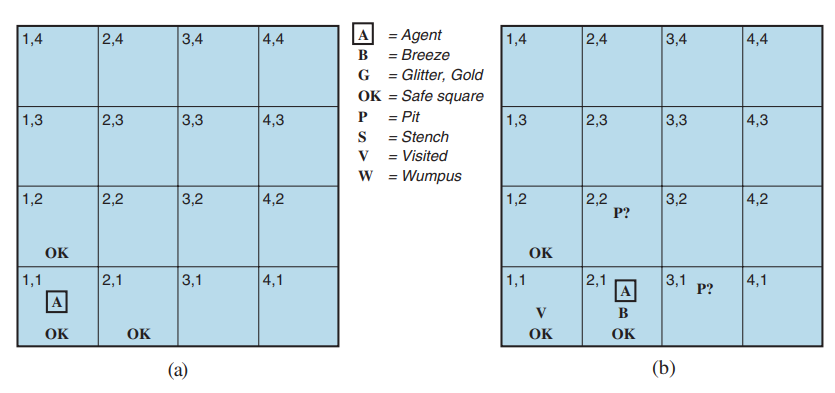
\includegraphics[scale=0.8]{images/wumpus-grid.png}
    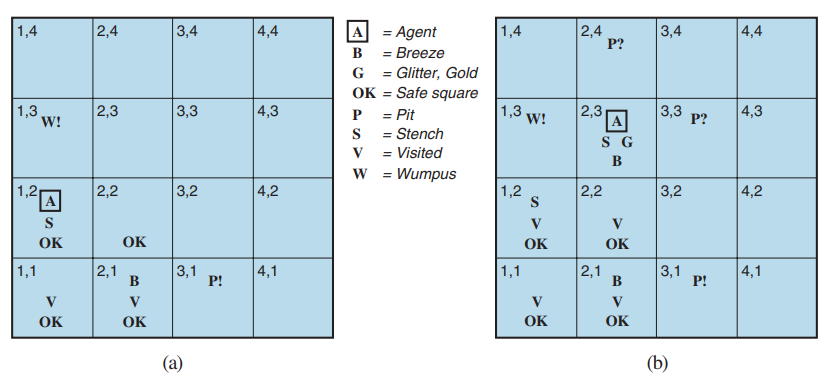
\includegraphics[scale=0.8]{images/wumpus-grid2.png}
\end{center}
Note that in each case for which the agent draws a conclusion from the available information, that conclusion is guaranteed to be correct if the available information is correct. we'll describe how to build logical agents that can represent in a \textbf{formal way} information and draw conclusions.

\section{Propositional Logic}
We now present a simple but powerful logic called \textbf{propositional logic}. The \textbf{syntax} of propositional logic defines the allowable sentences. The \textbf{atomic sentences} consist of a single proposition symbol (P, Q, R, ... but can be whatever). Each such symbol stands for a proposition that can be true or false. There are two proposition symbols with fixed meanings: \textit{True} is the always-true proposition and \textit{False} is the always-false proposition. \textbf{Complex sentences} are constructed from simpler sentences, using parentheses and \textbf{logical connectives}.
\begin{center}
    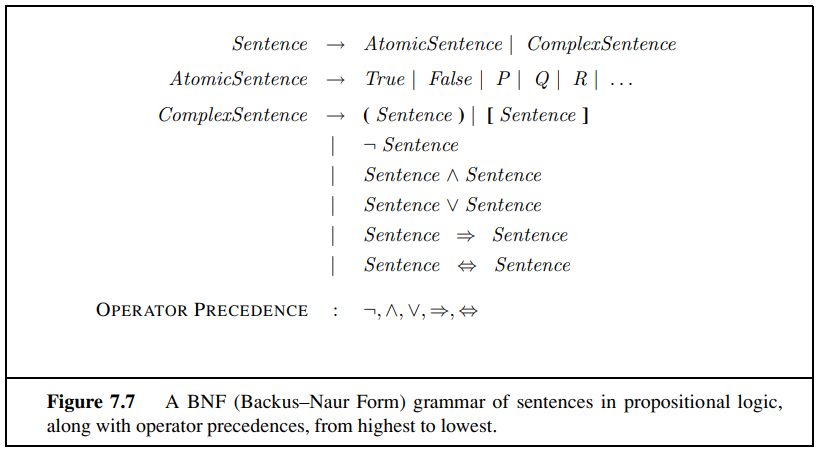
\includegraphics[scale=0.8]{images/BNF.png}
    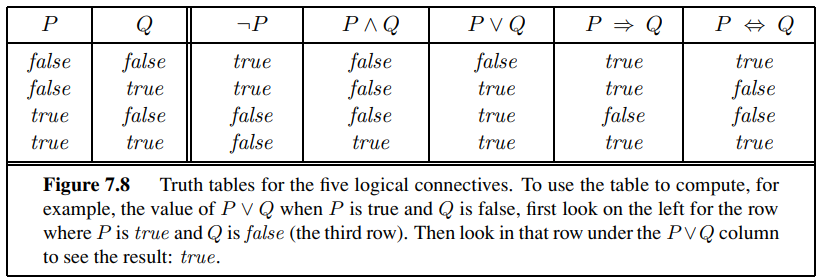
\includegraphics[scale=0.8]{images/truth-table.png}
\end{center}

\section{Models}
As we said previously, the knowledge bases consist of sentences. These sentences are expressed according to the \textbf{syntax} of the representation language, which specifies all the sentences that are well formed. A logic must also define the \textbf{semantics} or meaning of sentences. The semantics defines the truth of each sentence with respect to each possible world.\newline\newline
When we need to be precise, we use the term \textbf{model} in place of “possible world.”  If a sentence $\alpha$ is true in model $m$, we say that $m$ \textbf{satisfies} $\alpha$ or sometimes $m$ \textbf{is a model of} $\alpha$. We use the notation $M(\alpha)$ to mean the set of all models of $\alpha$. Basically, a model assigns truth values to proposition symbols of a sentence.\newline\newline
Now that we have a notion of truth, we are ready to talk about logical reasoning. This involves the relation of logical \textbf{entailment} between sentences, —the idea that a sentence follows logically from another sentence. In mathematical notation, we write:
\[\alpha \vDash \beta\]
to mean that the sentence $\alpha$ entails the sentence $\beta$. The formal definition of entailment is this: $\alpha \vDash \beta$ if and only if, in every model in which $\alpha$ is true, $\beta$ is also true. Using the notation just introduced, we can write
\[\alpha \vDash \beta\,\, \text{if and only if } M(\alpha) \subseteq M(\beta)\]
Note that the direction of the $\subseteq$ means that $\alpha$ is a stronger assertion than $\beta$.\newline\newline
We can apply the same kind of analysis to the wumpus-world reasoning example given previously. The agent has detected nothing in $[1,1]$ and a breeze in $[2,1]$. These percepts, combined with the agent’s knowledge
of the rules of the wumpus world, constitute the KB. The agent is interested (among other things) in whether the adjacent squares $[1,2]$, $[2,2]$, and $[3,1]$ contain pits. Each of the three squares might or might not contain a pit, so (for the purposes of this example) there are $2^3 = 8$ possible models.
\begin{center}
    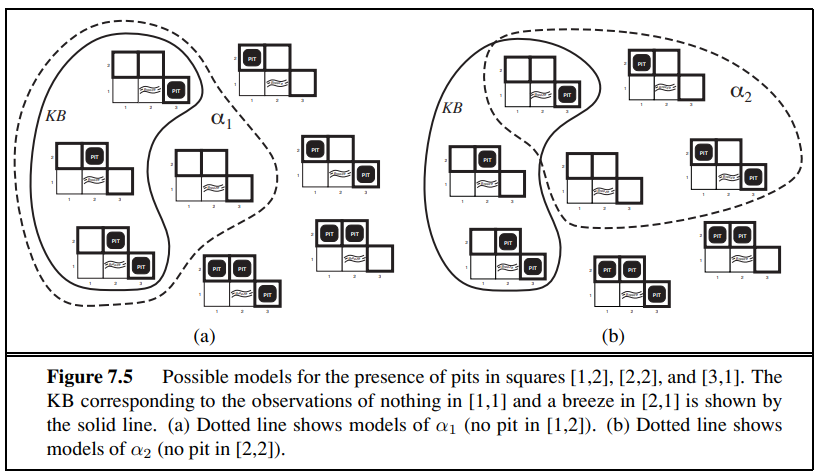
\includegraphics[scale=0.8]{images/kb-wumpus.png}
\end{center}
The KB can be thought of as a set of sentences or as a single sentence that asserts all the individual sentences. The KB is false in models that contradict what the agent knows; for example, the KB is false in any model in which $[1,2]$ contains a pit, because there is no breeze in $[1,1]$. There are in fact just three models in which the KB is true, and these are shown surrounded by a solid line in the figure above.\newline\newline
Now let us consider two possible conclusions:
\begin{itemize}
    \item $\alpha_1 = $ “There is no pit in $[1,2]$.”

    \item $\alpha_2 = $ “There is no pit in $[2,2]$.”

\end{itemize}
By inspection, we see the following: in every model in which KB is true, $\alpha_1$ is also true. Hence $KB \vDash \alpha_1$: there is no pit in $[1,2]$. We can also see that in some models in which KB is true, $\alpha_2$ is false. Hence, the agent cannot conclude that there is no pit in $[2,2]$.\newline\newline
In understanding entailment and inference, it might help to think of the set of all consequences of KB as a haystack and of $\alpha$ as a needle. Entailment is like the needle being in the haystack; inference is like finding it. This distinction is embodied in some formal notation: if an inference algorithm $i$ can derive $\alpha$ from KB, we write:
\[KB \vdash_i \alpha\]
which is pronounced “$\alpha$ is derived from KB by $i$”.\newline\newline
An inference algorithm that derives only entailed sentences is called \textbf{sound}: whenever $KB \vdash_i \alpha$, it is also true that $KB \vDash \alpha$. Note that, as we did with the example before, enumerating all possible models to check that $\alpha$ is true in all models in which KB is true is sound. The property of \textbf{completeness} is also desirable: an inference algorithm is complete if it can derive any sentence that is entailed.\newline\newline
If KB is true in the real world, then any sentence $\alpha$ derived from KB by a sound inference procedure is also true in the real world.

\section{A simple knowledge base}
Now we can construct a knowledge base for the wumpus world, focusing on its immutable aspects. For now, we need the following symbols for each $[x, y]$ location:
\begin{itemize}
    \item $P_{x, y}$ is true if there is a pit in $[x, y]$.
    \item $W_{x,y}$ is true if there is a wumpus in $[x, y]$, dead or alive.
    \item $B_{x,y}$ is true if the agent perceives a breeze in $[x, y]$.
    \item $S_{x,y}$ is true if the agent perceives a stench in $[x, y]$.
\end{itemize}
We label each \textbf{sentence} $R_i$ so that we can refer to them:
\begin{itemize}
    \item There is no pit in $[1,1]$: $R_1:\,\, \neg P_{1,1}$.
    \item A square is breezy if and only if there is a pit in a neighboring square. This has to be stated for each square; for now, we include just the relevant squares:
    \begin{itemize}
        \item $R_2: \,\, B_{1,1} \iff (P_{1,2} \lor P_{2, 1})$
        \item $R_3: \,\, B_{2,1} \iff (P_{1,1} \lor P_{2,2} \lor P_{3,1})$
    \end{itemize}

    \item The preceding sentences are true in all wumpus worlds. Now we include the breeze percepts for the first two squares visited in the specific world the agent is in, leading up to the situation in the figure above (Figure 7.5):
    \begin{itemize}
        \item $R_4: \,\, \neg B_{1,1}$
        \item $R_5: \,\, B_{2,1}$
    \end{itemize}
\end{itemize}
Our goal now is to decide whether $KB \vDash \alpha$ for some sentence $\alpha$. For example, is $\neg P_{1,2}$ entailed by our KB? Our first algorithm for inference is a \textbf{model-checking} approach that is a direct implementation of the definition of entailment: enumerate the models, and check that $\alpha$ is true in every model in which KB is true.
\begin{center}
    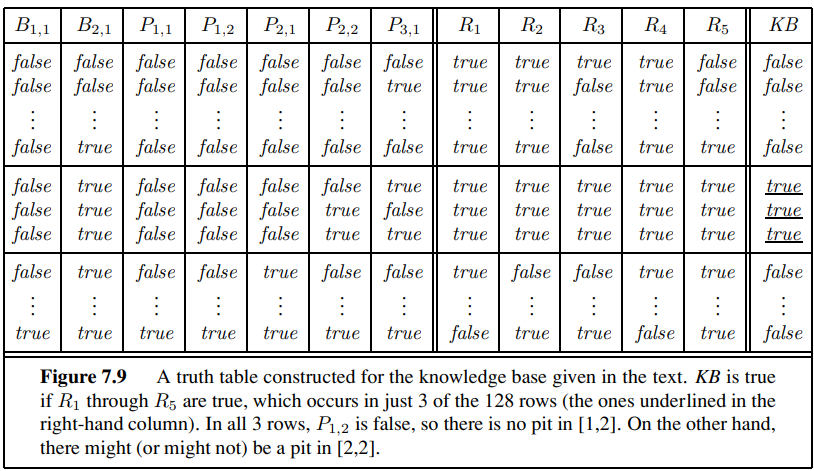
\includegraphics[]{images/wumpus-table.png}
\end{center}
Returning to our wumpus-world example, the relevant proposition \textbf{symbols} are $B_{1,1}, B_{2,1}, P_{1,1}, P_{1,2}, P_{2,1}, P_{2,2}$, and $P_{3,1}$. With seven symbols, there are $2^7 = 128$ possible models; in three of these, KB is true. Note that this is just a "snapshot" of the situation shown in the Figure 7.5. Obviously, as the agent goes on, the KB changes. In the three model where KB is \textit{True}, $\neg P_{1,2}$ is also \textit{True}. Hence, there is no pit in $[1,2]$. On the other hand, $P_{2,2}$ is true in two of the three models and false in one, so we cannot yet tell whether there is a pit in $[2,2]$. Note that KB is true if $R_1$ through $R_5$ are true (KB can be expressed as a sentence $R_1 \land ... \land R_5$), which occurs in just 3 of the 128 rows.
\begin{center}
    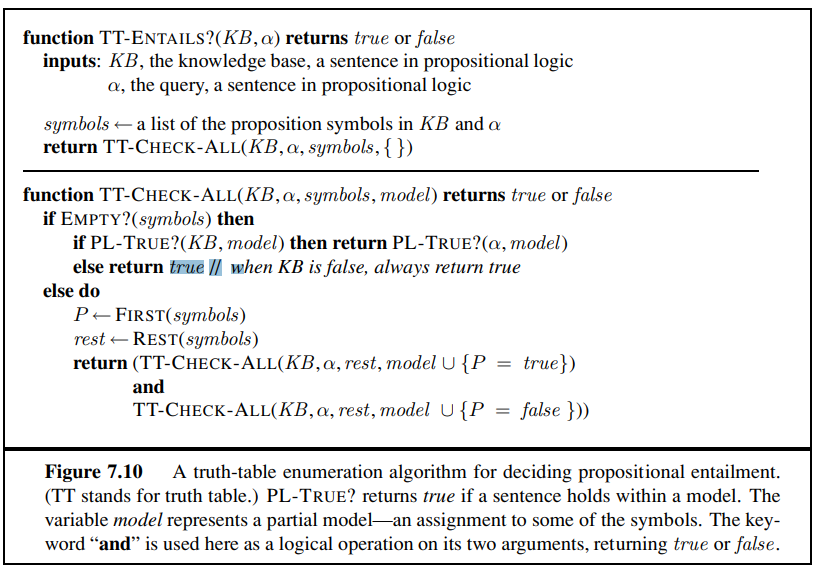
\includegraphics[]{images/tt-algorithm.png}
\end{center}
The algorithm above performs a recursive enumeration of a finite space of assignments to symbols. The algorithm is \textbf{sound} because it implements directly the definition of entailment, and \textbf{complete} because it works for any KB and $\alpha$ and always terminates; there are only finitely many models to examine.\newline\newline
Basically, the algorithm constructs the truth table seen above using a recursive implementation. In particular, it creates a binary tree where the nodes are the symbols in the KB and the branches are truth assignment for that symbol (\textit{True} or \textit{False}). It starts from the first symbol and recursively produces all the possible assignment for all the possible symbols. The paths from the root to the leaves corresponds to the rows of the table above, i.e. the models. Once the algorithm arrives at a leaf, it checks whether the sentence $\alpha$ holds within the corresponding model (path). The algorithm returns always \textit{True} if the KB is \textit{False} w.r.t the model because we are only interested to see if a sentence is \textit{True} when the KB is \textit{True}. These operations correspond to look at the rows of the table (models) where KB is \textit{True} and check whether $\alpha$ is also \textit{True}. If the sentence $\alpha$ is \textit{True} for all the models where also KB is \textit{True} (i.e. all the leaves \textit{returns} \textit{True}), then $\alpha$ can be deduces from KB. Note that if all the leaves return \textit{True}, when the algorithm ascents from recursion, the \textit{True} value is propagated towards the root by the logical \textit{and} and eventually the algorithm returns \textit{True}.  For the same reason, it is sufficient that just one leaf returns \textit{False} that the whole algorithm returns \textit{False} (this is why the algorithms always returns \textit{True} when KB is \textit{False}).\newline\newline
Note that If KB and $\alpha$ contain $n$ symbols in all, then there are $2^n$ models. Thus, the time complexity of the algorithm is $O(2^n)$ (The space complexity is only $O(n)$ because the enumeration is depth-first). Unfortunately, propositional entailment is co-NP-complete.
